\subsection{Mapping a concrete \alert{Topic-Level Hierarchy} into \alert{JSON-Format}}

\begin{frame}[fragile]{Mapping of a concrete \alert{Topic-Level Hierarchy} into MQTTSuites \alert{JSON-Format}}
\begin{columns}[]
\begin{column}{0.5\textwidth}
\begin{figure}
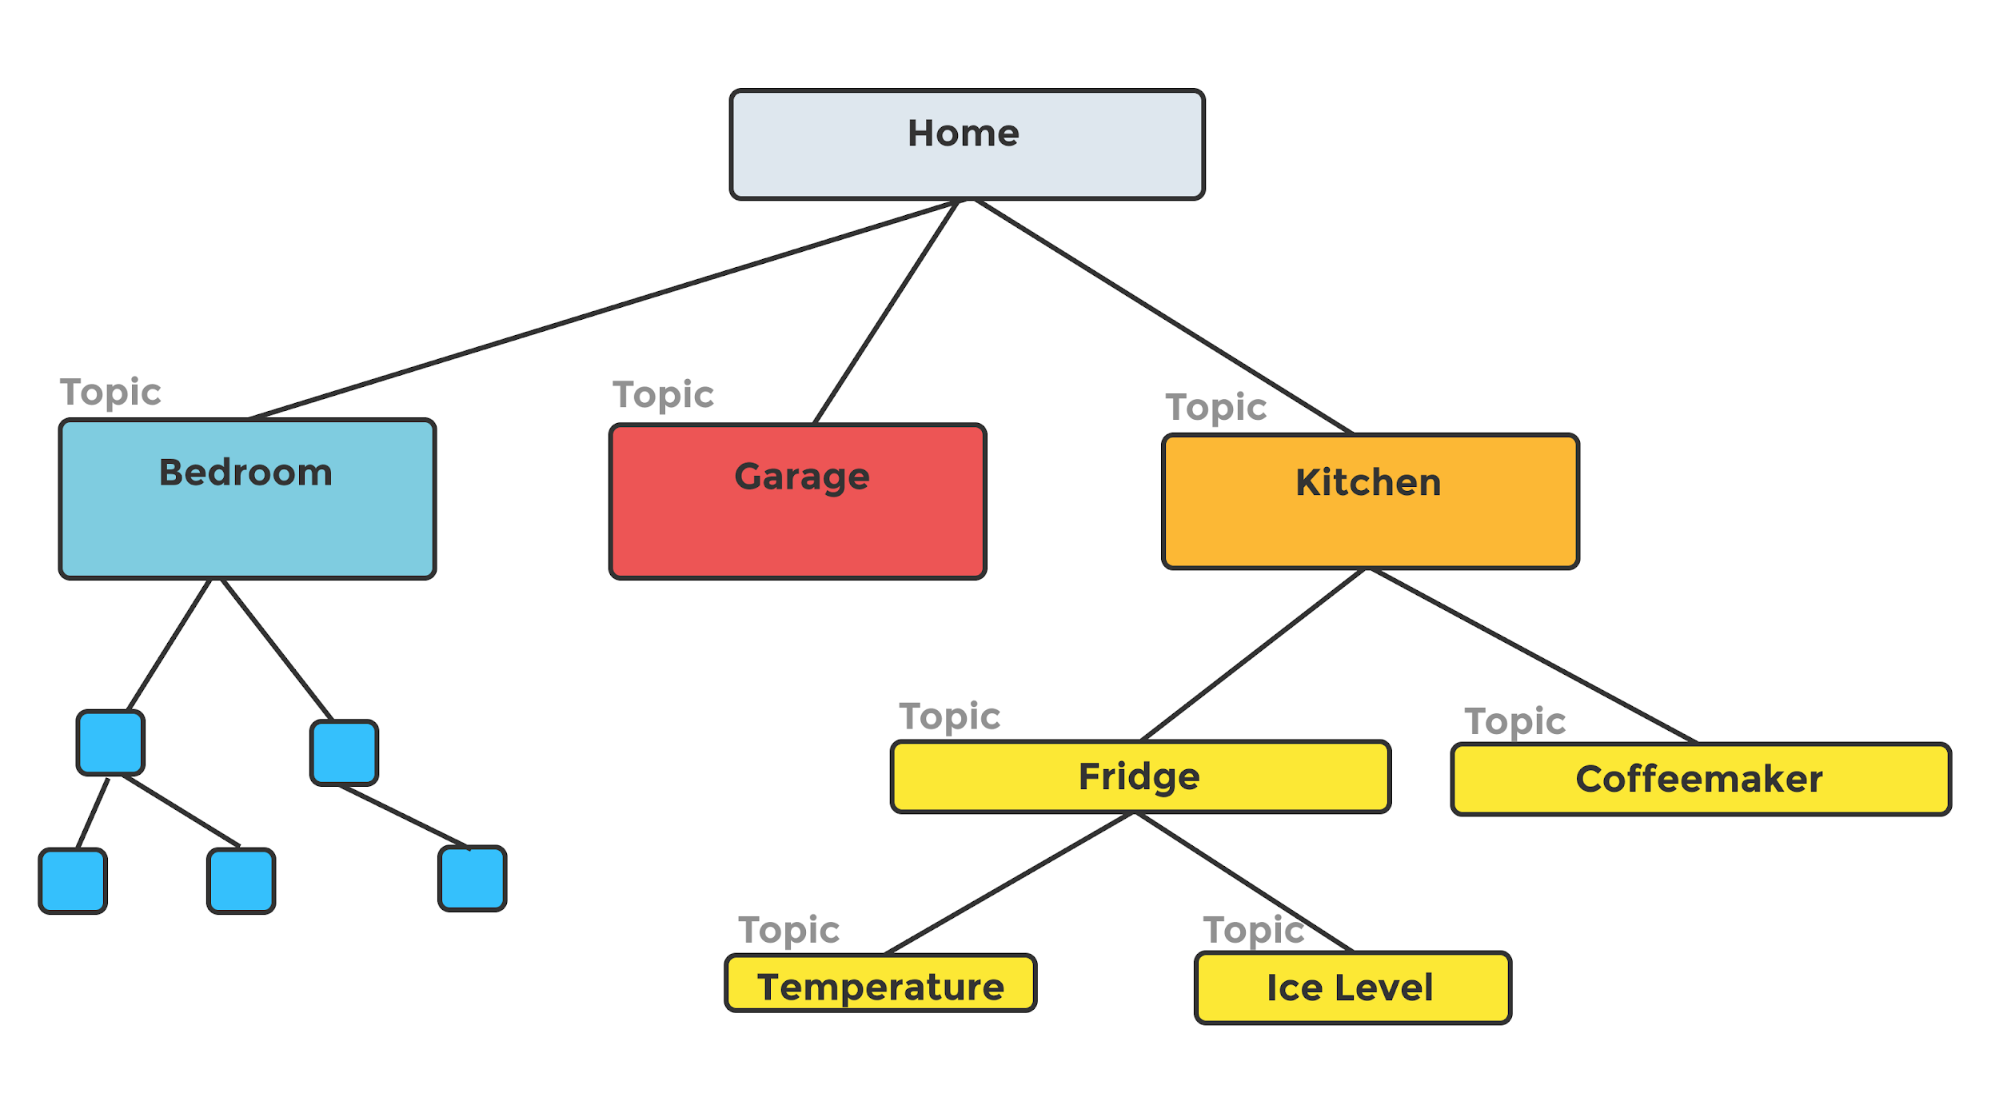
\includegraphics[scale=0.11]{images/mqtt-topics.png}
\vskip-1em
\caption{A topic-level hierarchy.\\\tiny From: \href{https://www.cloudmqtt.com/blog/the-mqtt-beginners-guide-what-is-mqtt.html}{https://www.cloudmqtt.com/blog/the-mqtt-beginners-guide-what-is-mqtt.html}}
\vskip-0.8em
\end{figure}
\begin{scriptsize}
\begin{Verbatim}
Home/Bedroom/...
Home/Bedroom/.../...
Home/Garage
Home/Kitchen/Fridge/Temperature
Home/Kitchen/Fridge/IceLevel
Home/Kitchen/Coffemaker
\end{Verbatim}
\end{scriptsize}
\end{column}
\begin{column}{0.3\textwidth}
  \begin{jsoncode}[autogobble=true,basicstyle=\tiny\codefontfamily,]
      "mapping" : {
          "topic_level" : {
              "name" : "Home",
              "topic_level" : [{
                  "name" : "Bedroom",
                  "topic_level" : [{
                      "name" : "...",
                  }, {
                      "name" : "...",
                  }],
              },
              {
                  "name" : "Garage",
              },
              {
                  "name" : "Kitchen",
                  "topic_level" : [{
                      "name" : "Fridge",
                      "topic_level" : [{
                          "name" : "Temperature",
                      },
                      {
                          "name" : "IceLevel",
                      }],
                  },
                  {
                      "name" : "Cofffmaker",
                  }],
              }],
          }
      }
  \end{jsoncode}
\end{column}
\end{columns}
\end{frame}

